\documentclass{article}

\usepackage[utf8]{inputenc}
\usepackage[spanish]{babel}

\usepackage{geometry}               % Márgenes del documento
\usepackage{amsfonts}
\usepackage{graphicx}

\usepackage{tabularx}

\usepackage{amsthm} % para teoremas y lemas

\usepackage[nottoc]{tocbibind}

\usepackage{color}
\usepackage[pdftex, colorlinks=true, linkcolor=blue, urlcolor=red, filecolor=magenta, citecolor=blue]{hyperref}
\definecolor{gray97}{gray}{.97}
\definecolor{gray95}{gray}{.95}
\definecolor{gray75}{gray}{.75}
\definecolor{gray45}{gray}{.45}

\usepackage{listings}
\usepackage[usenames,dvipsnames]{xcolor}
\colorlet{keyword}{blue!100!black!80}
\colorlet{STD}{Lavender}
\colorlet{comment}{green!80!black!90}

\lstset{ %
	backgroundcolor = \color{gray95},
	breaklines=true,
	numbers=left,
	numbersep=5pt,
	tabsize=3,
	commentstyle=\color{comment},
	showstringspaces=false,
	numberstyle=\tiny\color{gray45}
}

\lstdefinestyle{xml}{
	language     = XML, %basicstyle=\ttfamily\footnotesize,
	morestring=[b]",
	moredelim=[s][\bfseries\color{Maroon}]{<}{\ },
	moredelim=[s][\bfseries\color{Maroon}]{</}{>},
	moredelim=[l][\bfseries\color{Maroon}]{/>},
	moredelim=[l][\bfseries\color{Maroon}]{>},
	morecomment=[s]{<?}{?>},
	morecomment=[s]{<!--}{-->},
	stringstyle=\color{blue},
	identifierstyle=\color{red},		
	frame=single, % Se pone un marco
	basicstyle   = \footnotesize \ttfamily,
	keywordstyle = [1]\color{keyword}\bfseries,
	keywordstyle = [2]\color{STD}\bfseries
}

\lstdefinestyle{java}{
	language     = Java,
	frame=single, % Se pone un marco
	basicstyle   = \footnotesize \ttfamily,
	keywordstyle = [1]\color{keyword}\bfseries,
	keywordstyle = [2]\color{STD}\bfseries,
	breaklines=true,                % sets automatic line breaking
	commentstyle = \color{comment}
}

\lstdefinestyle{sql}{
	language     = SQL,
	frame=single, % Se pone un marco
	basicstyle   = \footnotesize \ttfamily,
	keywordstyle = [1]\color{keyword}\bfseries,
	keywordstyle = [2]\color{STD}\bfseries,
	breaklines=true,                % sets automatic line breaking
	commentstyle = \color{comment}
}

\lstdefinestyle{bash}{
	language     = bash,
	frame=none, % Se pone un marco
	showstringspaces=false, % No muestre el cuadrado en los espacios de los strings
	basicstyle   = \footnotesize \ttfamily,
	keywordstyle = [1]\color{keyword}\bfseries,
	keywordstyle = [2]\color{STD}\bfseries
}

\geometry{a4paper}                  % Tamaño y márgenes del documento
\geometry{left=2.5cm,top=2.5cm}
\geometry{bottom=2.5cm,right=2.5cm}

\geometry{driver=dvips,pdftex} % ???
\setcounter{secnumdepth}{5}    % ???
\setcounter{tocdepth}{5}       % ???

\setlength{\parskip}{\baselineskip} % Espacio entre párrafos (una linea en blanco)

%--------------------------------------------------------------------------
\title{\textbf{Tutorial de Hibernate 4.3.8.Final}}
%\author{flanciskinho}
\date{} %Asi no inserta la fecha


\begin{document}


\maketitle % Pone titulo, autor

\renewcommand{\abstractname}{Abstract} % El nombre que aparece al principio del abstract
\begin{abstract}
	Este documento pretende ser una pequeña guía de como empezar a usar la version \emph{4.3.8.Final} de Hibernate.
\end{abstract}

\renewcommand{\contentsname}{} % Lo que pone en el indice
{\setlength{\parskip}{0mm} \tableofcontents} % Para que no ponga espacios entre las lineas de indice

%\vspace{2cm} % Para dejar un espacio con respecto a la tabla
\newpage

\section{Introducción}


\section{Commit 1. Empezando con el proyecto}

\subsection{Preparando la BBDD}
	Lo primero que vamos a realizar en este paso es preparar la base de datos sobre la que trabajar. En este caso se usará MySQL que tendrá una base de datos \emph{pojo}.
\begin{lstlisting}[style=bash]
	mysqladmin -u root create pojo
\end{lstlisting}

	Lo siguiente es poder permitir el acceso a un usuario \emph{pojo} que tendrá como contraseña \emph{pojo}
\begin{lstlisting}[style=bash]
	mysql -u root
	
	mysql> GRANT ALL PRIVILEGES ON pojo.* to pojo@localhost IDENTIFIED BY 'pojo';
\end{lstlisting}

\subsection{Creando el proyecto con maven}
	Para la creación del proyecto con Maven se introduce el siguiente código por terminal
\begin{lstlisting}[style=bash]
mvn archetype:generate -DgroupId=org.example.tutorials.hibernate -DartifactId=hibernateTutorial -DarchetypeArtifactId=maven-archetype-quickstart -DinteractiveMode=false
\end{lstlisting}

Esto nos genera un archivo pom.xml muy pobre como el que se ve a continuación:
\lstinputlisting[style=xml]{commit01/code/pomInicial.xml}

Para poder trabajar con Hibernate lo modificaremos por algo así:
\lstinputlisting[style=xml]{commit01/code/pom.xml}

A mayores también creamos las carpetas para almacenar los recursos
\begin{lstlisting}[style=bash]
mkdir -p src/main/resources/org/example/tutorials/hibernate/hibernateTutorial
\end{lstlisting}

\subsection{Creando una tabla para los eventos}
	Para poder dotar de persistencia a los datos necesitamos tener un sitio donde poder guardar los datos nuevos y poder recuperar los datos viejos así que para eso creamos un archivo sql que genere una tabla para guardar eventos
\lstinputlisting[style=sql]{commit01/code/01-CreateTables.sql}

	Como podemos ver en el archivo sql, la tabla eventos almacena instancias de eventos que tendrán un identificador (que no es más que un entero), una fecha (que es una fecha) y un título (que es una cadena de caracteres).

	Si suponemos que el archivo se encuentra en la ubicación \emph{src/sql/01-CreateTables.sql} basta con introducir el siguiente comando para ejecutarlo en el gestor
\begin{lstlisting}[style=bash]
 mysql pojo -u pojo -p < src/sql/01-CreateTables.sql
\end{lstlisting}

\subsection{Creando el objeto Evento}
	La idea ahora es poder usar los Eventos que se encuentren en la base de datos en nuestro código Java. Así que para eso creamos una clase como la siguiente:
\lstinputlisting[style=java]{commit01/code/Event.java}

	Como podemos ver, la clase \emph{Event} tiene los atributos necesarios para poder guardar almacenar una fila de la tabla \emph{events}.

\subsection{Como indicar la relación entre la clase y la tabla}
	Como hemos visto hasta ahora no se ha indicado en ningún lado como se realiza el mapeo de los objetos con la BBDD, en este apartado se creará un archivo para indicar esta relación.
	
	El fichero para indicar esta relación como pasar de la BBDD a los objetos en Java se guarda en la ruta \emph{src/main/resources/org/example/tutorials/hibernate/hibernateTutorial/domain/} bajo el nombre de \emph{Event.hbm.xml} y tiene que tener el siguiente contenido:
\lstinputlisting[style=xml]{commit01/code/Event.hbm.xml}

	Como podemos ver el elemento \emph{hibernate-mapping} es el que contiene la información de como es la relación entre la clase hecha en java y la tabla de la BBDD. El atributo \emph{package} del elemento \emph{hibernate-mapping} es el paquete a donde pertenece la clase. Dentro de ese elemento está el elemento \emph{class} que tiene los siguientes atributos
{\setlength{\parskip}{0mm}
\begin{itemize}
	\item \emph{name} Que es el nombre de la clase java
	\item \emph{table} Es el nombre de la tabla en la BBDD
\end{itemize}
}
	
	Dentro del elemento \emph{class} se indican los atributos con el elemento \emph{property} que tiene tres elementos:
{\setlength{\parskip}{0mm}
\begin{itemize}
	\item \emph{name} que es el nombre del atributo en la clase java
	\item \emph{column} que es el nombre de la columna de la tabla que hay en la BBDD
	\item \emph{type} Es el tipo de dato que hibernate\cite{{HibernateData}} usa para tratar con esos objetos (no son tipos de datos Java ni tipos de datos SQL)
\end{itemize}
}

	Como podemos ver en el fichero hay un elemento llamado \emph{id}. Este elemento se usa para indicar cual es la clave y tiene la misma sintaxis que el elemento \emph{property}. Además a mayores se le puede especificar la forma en la que se genera esta clave (en el fichero indicamos que es la BBDD la que se encarga de asignarle el valor adecuado).
	
\subsection{Configurando hibernate}
	Una de las cosas que nos hace falta es indicar a hibernate como acceder a la BBDD, para ello creamos el archivo \emph{hibernate.cfg.xml} en la ruta \emph{src/main/resources} con la siguiente información:
\lstinputlisting[style=xml]{commit01/code/hibernate.cfg.xml}

	Como podemos ver, este es el fichero que indica a hibernate como conectarse a la base de datos para poder trabajar con ella. Las propiedades que hay en el fichero de configuración son:
{\setlength{\parskip}{0mm}
\begin{itemize}
	\item \emph{connection.driver\_class} Indica el driver JDBC a usar. Esto no lo descarga, sólo indica cual es, por eso en el archivo pom.xml está especificado que se incluya esa librería en el código
	\item \emph{connection.url} Es la cadena de conexión con la BBDD
	\item \emph{connection.username} Es el nombre de usuario con el que se accede a la BBDD
	\item \emph{connection.password} Contraseña del usuario con el que se accede a la BBDD
	\item \emph{connection.pool\_size} Indica cuantas conexiones están abiertas con la BBDD
	\item \emph{dialect} Es el lenguaje específico de SQL que tiene que usar Hibernate contra la BBDD
	\item \emph{show\_sql} Para mostrar por la salida estándar las consultas que realiza hibernate 
\end{itemize}
}

	A mayores hay un elemento más, el elemento \emph{mapping}, que es con el que indicamos que clases tienen equivalencias con las tablas en la BBDD.

\subsection{Una ayuda para las sesiones de hibernate}
	Las forma de trabajar con una BBDD es estableciendo primero una sesión con ella. Para hacer el código más sencillo creamos una clase llamada \emph{HibernateUtil.java} cuyo código se puede ver a continuación
\lstinputlisting[style=java]{commit01/code/HibernateUtil.java}

	Lo que realiza este código es devolvernos un objeto único que será el encargado de dar acceso al resto del API de hibernate.
	
\subsection{Usando hibernate}
	Una vez llegados a este punto tenemos todo listo para empezar a trabajar con objetos persistentes. Para ello creamos la clase \emph{App.java} que tiene ejemplos de ciertas operaciones:
\lstinputlisting[style=java]{commit01/code/App.java}

	Podemos ver que lo primero que se realiza antes de empezar con una operación es abrir una sesión a partir del objeto que nos devuelve \emph{HibernateUtil.getSessionFactory}. El siguiente paso es iniciar una transacción sobre el que se van a realizar operaciones con la base de datos. En el caso de que todo sea correcto, la transacción acaba con un \emph{commit}, pero si Hibernate nos devuelve una excepción deshacemos los cambios con un \emph{rollBack}. Al final de todo cerramos la sesión que hemos abierto para trabajar con la BBDD.

	Para ejecutar el código basta con introducir el siguiente comando en la terminal:
\begin{lstlisting}[style=bash]
mvn clean compile exec:java -Dexec.mainClass=org.example.tutorials.hibernate.hibernateTutorial.App
\end{lstlisting}

\subsection{Estado del sistema}
	Al final de esta iteración lo que tenemos es algo como lo que se muestra en la figura \ref{fig:c01:UmlClass}.
\begin{figure}[h]
  \centering
    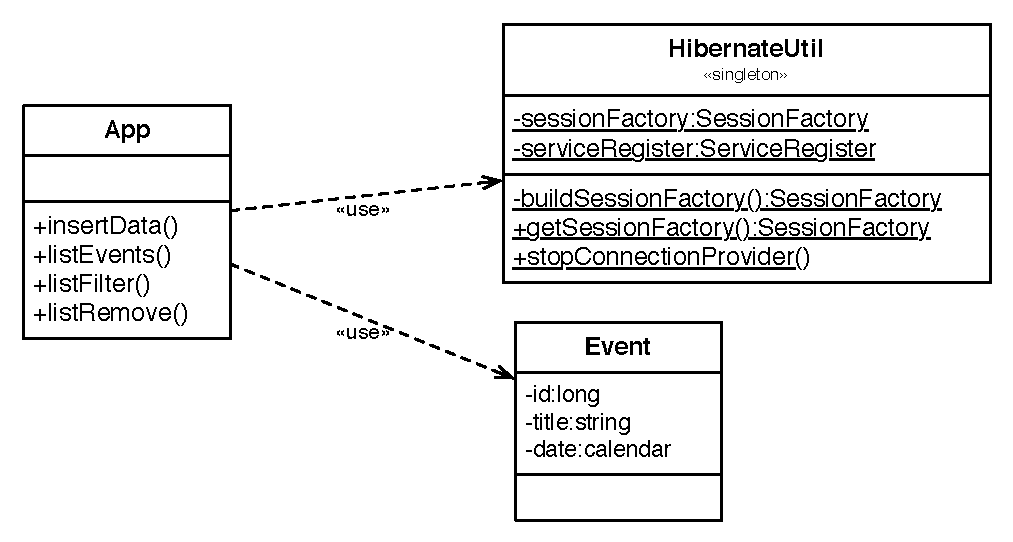
\includegraphics[width=0.7\textwidth]{commit01/img/UmlClass.pdf}
  \caption{Diagrama de clases}
  \label{fig:c01:UmlClass}
\end{figure}	
	
\section{Commit 2. Ordenando el código}\label{sec:commit2}
	En la iteración anterior se puso en marcha un ejemplo sencillo para empezar a usar Hibernate y aunque funciona el código este no es estructuralmente correcto. Sería más correcto tratar de ocultar los mecanismos de persistencia de los datos ya que la lógica de negocio tendría que ser independiente del método de persistencia se empleé (debería de dar igual si se usa un SGBD, un archivo plano...). Para estos casos se usa un patrón conocido como DAO\cite{Dao}.

\begin{figure}[h]
  \centering
    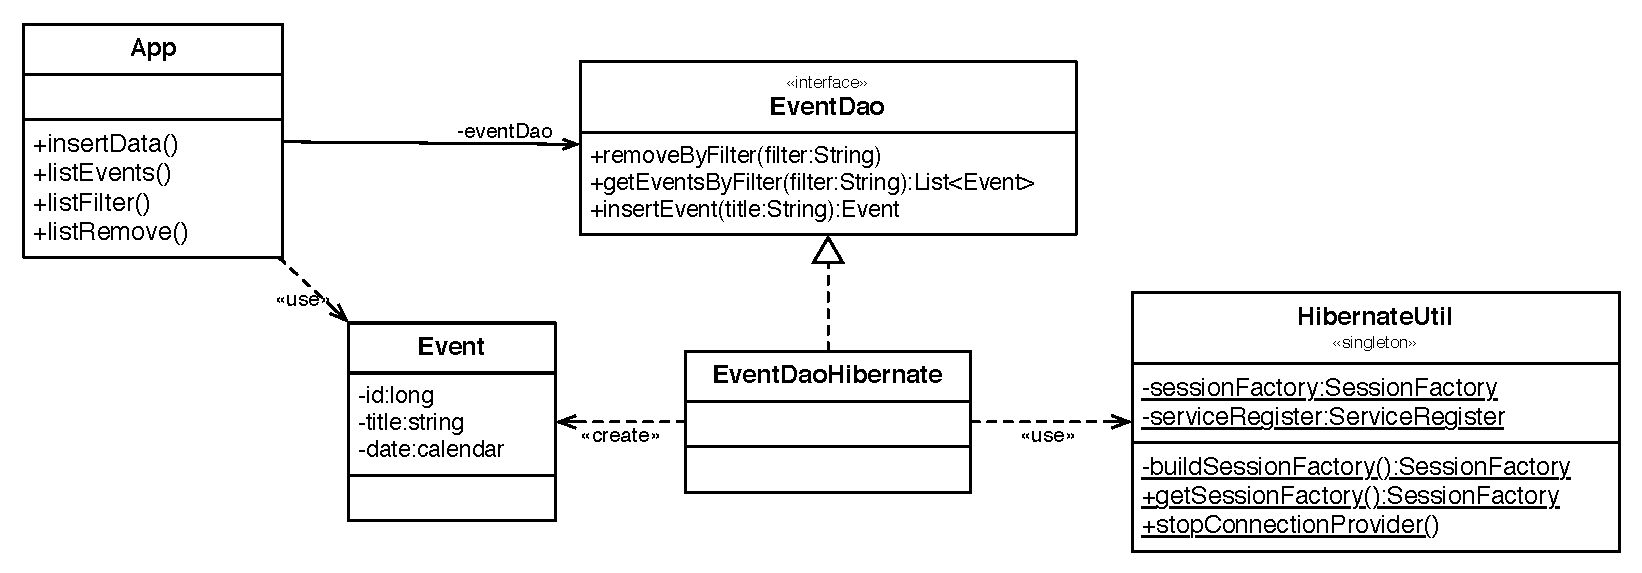
\includegraphics[width=0.9\textwidth]{commit02/img/UmlClass.pdf}
  \caption{Diagrama de clases}
  \label{fig:c02:UmlClass}
\end{figure}	

\subsection{Implementación del patrón DAO}
	El objetivo de esta iteración es implementar el patrón DAO para el uso de los eventos. La idea es que al final tengamos algo como en la imagen \ref{fig:c02:UmlClass}. Como podemos ver en la imagen \ref{fig:c02:UmlClass} la clase \emph{App} que es lo que sería la lógica de negocio no sabe que mecanismo de persistencia se está empleando, el solo hace las peticiones a través de una interfaz llamada \emph{EventDao}. La implementación de la interfaz, que en este caso es \emph{EventDaoHibernate}, es la encargada de usar los mecanismos de persistencia necesarios y funciona como una caja negra. La clase \emph{EventDaoHibernate} funciona como una caja negra ya que es quien trata la persistencia de los objetos \emph{Event}. La ventaja de usar este patrón es que si el día de mañana cambian la manera de tratar los datos basta con realizar la implementación adecuada de la interfaz \emph{EventDao} para que todo funcione correctamente.
	
	La interfaz \emph{EventDao} queda de la siguiente manera:
\lstinputlisting[style=java]{commit02/code/EventDao.java}

	La implementación de la interfaz del DAO (\emph{EventDaoHibernate}) queda de la siguiente manera:
\lstinputlisting[style=java]{commit02/code/EventDaoHibernate.java}

	La otra clase que se ha modificado para un uso adecuado ha sido la clase \emph{App}:
\lstinputlisting[style=java]{commit02/code/App.java}

\section{Commit 3. Don't Repeat Yourself}
	Como hemos podido ver en la iteración anterior, se puede separar la parte que se encarga de realizar las operaciones de persistencia con el resto del código. Pero como podemos ver en la imagen \ref{fig:c03:Dry} se está repitiendo información (que exactamente lo dice el principio DRY\footnote{ \textit{Don't repeat yourself} \url{http://es.wikipedia.org/wiki/No_te_repitas}} que no hagamos).

\begin{figure}[h]
  \centering
    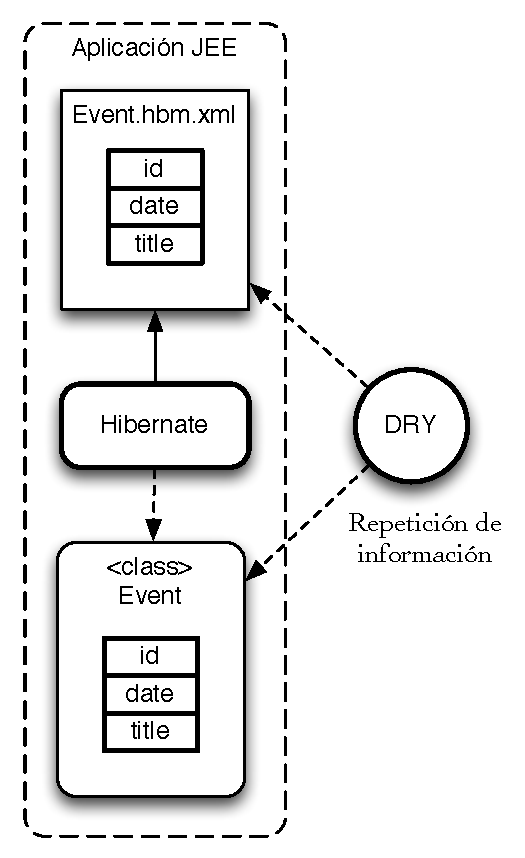
\includegraphics[width=0.25\textwidth]{commit03/img/Dry.pdf}
  \caption{Repetición de información en Hibernate}
  \label{fig:c03:Dry}
\end{figure}	

	La forma de evitar repetir la información es que se unifique lo que hay en el fichero de recurso \emph{Event.hbm.xml} con lo que hay en la clase \emph{Event.java}. El problema de realizar esto es que en la clase persistente metemos información que no está relacionada con ella (cosa que rompe el principio que se evitó en la iteración anterior). Esto nos lleva a tener que eligir tener un problema y sólo una solución:
{\setlength{\parskip}{0mm}
\begin{enumerate}
	\item Tener la parte de la persistencia separada del código y tener información repetida.
	\item No repetir información y tener parte de como se lleva a cabo la fuera de la zona que ``debería'' estar.
\end{enumerate}
}
	La opción que se suele escoger es la segunda por dos motivos. Uno es que no es habitual cambiar el método de persistencia (no se suele cambiar de SGBD) y la repetición de información puede tener grandes problemas de mantenimiento.
	
\subsection{Cambio del fichero hbm.xml por anotaciones}
	La forma de tener unificada la información del fichero \emph{Event.hbm.xml} y la clase \emph{Event.java} es usando anotaciones.
	
	El primer paso a realizar es eliminar el fichero \emph{Event.hbm.xml}; por eso hay que eliminar del fichero \emph{hibernate.cfg.xml} la referencia a ese fichero que era la siguiente línea:
\begin{lstlisting}[style=xml]
<mapping
    resource="org/example/tutorials/hibernate/hibernateTutorial/domain/Event.hbm.xml"/>
\end{lstlisting}
pero hay que indicarle que ahora hay una clase persistente (cuya información de persistencia está incluida en ella), lo que se indica de la siguiente manera:
\begin{lstlisting}[style=xml]
<mapping class="org.example.tutorials.hibernate.hibernateTutorial.domain.Event"/>
\end{lstlisting}

	Ahora en la clase \emph{Event.java} hay que indicar mediante anotaciones lo que había en el fichero \emph{Event.hbm.xml} de tal manera que queda algo tal que así:
\lstinputlisting[style=java]{commit03/code/Event.java}

	Lo primero que hay que hacer es indicar que eso es una clase persistente. Eso se especifica con la Anotación \emph{@Entity} encima de la declaración de la clase. También indicamos el nombre de la tabla con la anotación \emph{@Table(name =``EVENTS'')} donde \emph{EVENTS} es el nombre de la tabla con el que se realizará el mapeo. La forma de indicar que métodos trabajan con que columnas es con la etiqueta \emph{@Column(name = ``EVENT\_DATE'')} donde \emph{EVENT\_DATE} es el nombre de la columna sobre la que se realizan las operaciones en la BBDD. Por último para indicar cual es el identificador de la tabla basta con añadir la anotación \emph{@Id}. Normalmente los identificadores los genera el propio SGBD que tienen dos maneras de hacerlo
{\setlength{\parskip}{0mm}
\begin{enumerate}
	\item Mediante secuencias (como por ejemplo Oracle)
	\item Mediante identificadores autoincrementales (como MySQL)
\end{enumerate}
}

	En este caso estamos usando la segunda opción que se indica con la anotación \emph{@GeneratedValue(strategy = ``GenerationType.IDENTITY'')}. Para el segundo caso habría que poner algo del estilo:
\begin{lstlisting}[style=java]
@Column(name ="EVENT_ID")
@SequenceGenerator(          // It only takes effect for
  name = "EventIdGenerator", // databases providing identifier
  sequenceName = "EventSeq") // generators.
@Id
@GeneratedValue(strategy = GenerationType.SEQUENCE, generator = "EventIdGenerator")
\end{lstlisting}

	Una de las cosas por la que también nos decantamos por unificar la información del fichero \emph{Event.hbm.xml} y la clase \emph{Event.java} es que aunque se introduce información en la clase persistente no se introduce información del ORM que estamos usando, de tal manera que sólo las implementaciones de las interfaces de los DAOs saben que ORM están usando.

\section{Commit 4.  Empezando a relacionarse}

	Hasta ahora hemos empezado a usar hibernate con solo una clase persistente, lo que no es muy realista. Lo normal es que exista más de una clase persistente y existan ciertas relaciones entre ellas. En este aparatado vamos a incluir los eventos en una categoría.

\subsection{Modelado}
\begin{figure}[h]
  \centering
    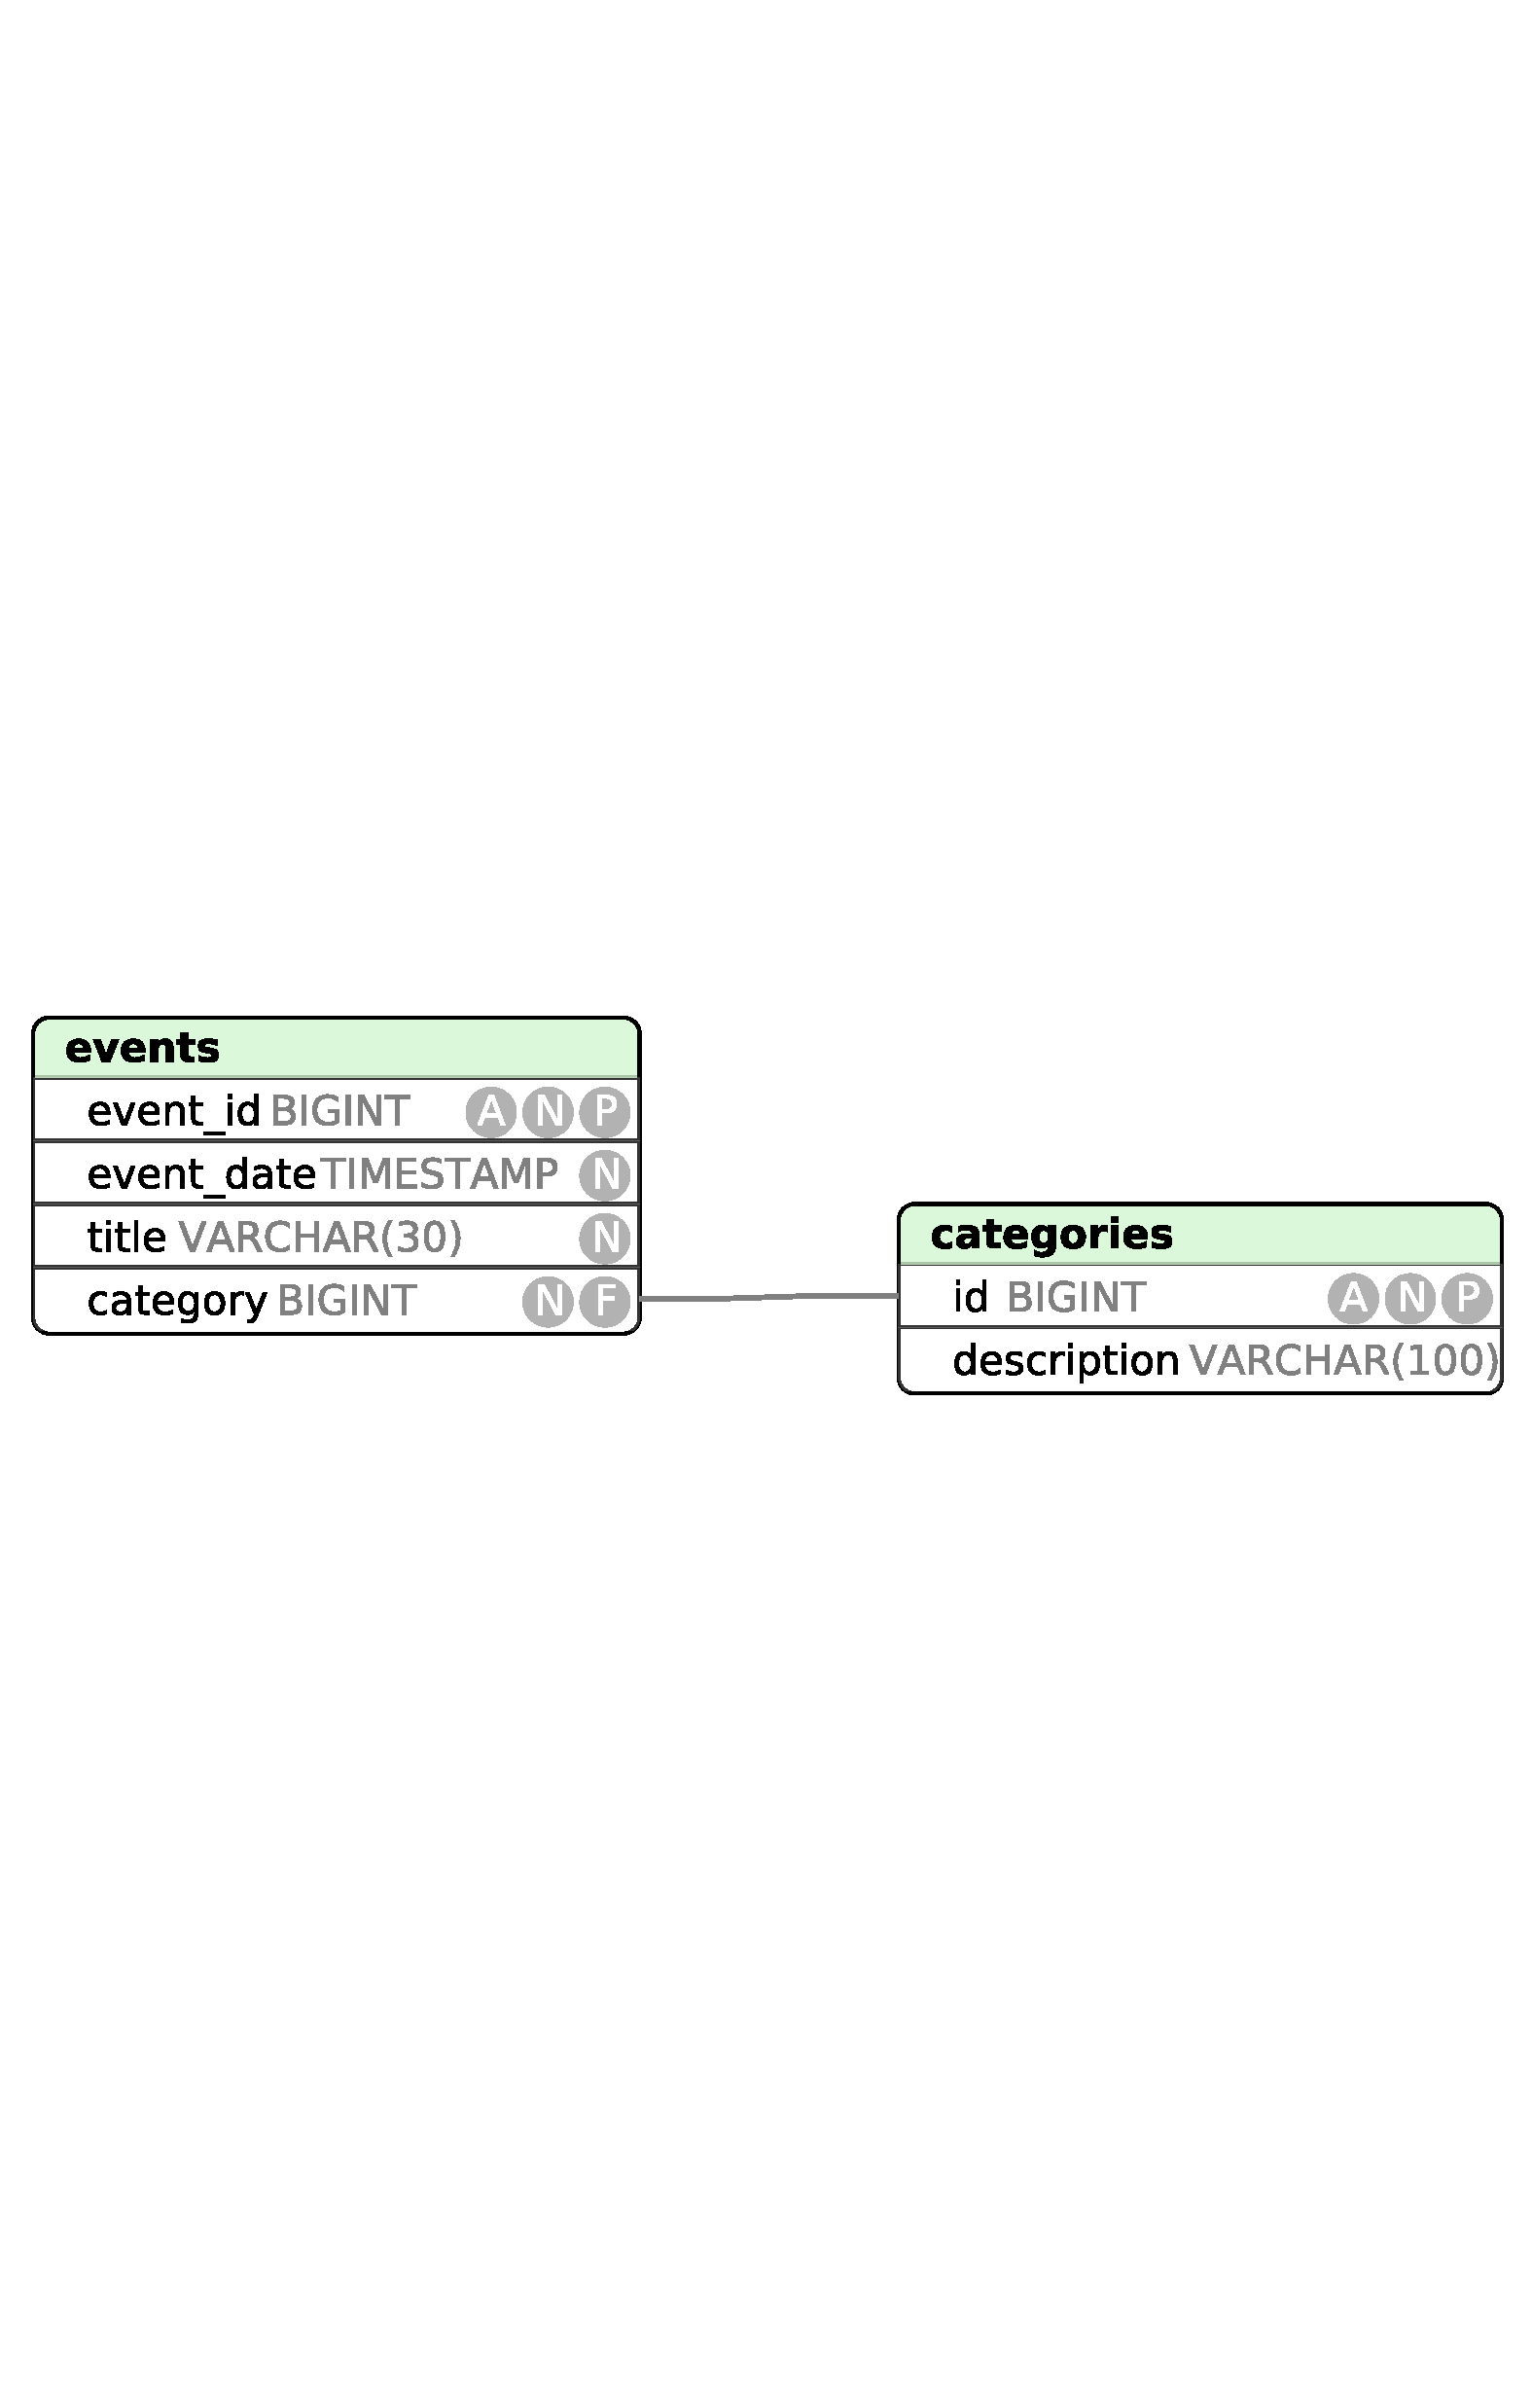
\includegraphics[width=0.5\textwidth]{commit04/img/ER.pdf}
  \caption{Diagrama entidad relación}
  \label{fig:c04:ER}
\end{figure}	

	Al clasificar los eventos el gráfico relacional nos quedaría como se muestra en la figura \ref{fig:c04:ER} en donde podemos ver, que a la hora de implementarlo como clases persistentes, podemos poner que el evento está asociado a una categoría y que una categoría tiene una lista de eventos. Realmente lo que se hace es modelar que los eventos pertenecen a una categoría. La parte en la que se indica mediante un atributo una lista de eventos no se modela porque una categoría puede tener millones de eventos, lo que al traerlos de la BBDD supone un gran coste para que después, muy probablemente, no se lleguen a usar.
	
	Así pues el diagrama de clases para representar los eventos y las categorías quedaría como se muestra en la imagen \ref{fig:c04:EventCategory}.

\begin{figure}[h]
  \centering
    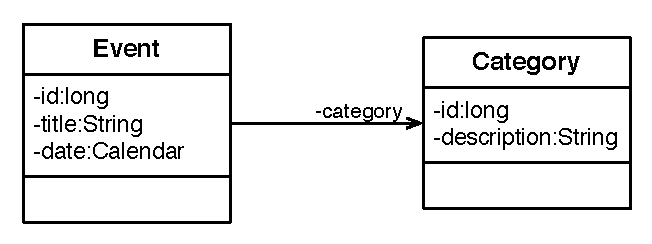
\includegraphics[width=0.5\textwidth]{commit04/img/EventCategory.pdf}
  \caption{Representación de los eventos y las categorías}
  \label{fig:c04:EventCategory}
\end{figure}	

\subsection{Codificación}

\subsubsection{BBDD}
	Así entonces lo primero que hacemos es modificar el archivo que crea las bases de datos:
\lstinputlisting[style=sql]{commit04/code/01-CreateTables.sql}

	Si suponemos que el archivo se encuentra en la ubicación \emph{src/sql/01-CreateTables.sql} basta con introducir el siguiente comando para ejecutarlo en el gestor:
\begin{lstlisting}[style=bash]
 mysql pojo -u pojo -p < src/sql/01-CreateTables.sql
\end{lstlisting}

\subsubsection{Java}
	Es hora de crear la clase persistente en nuestro código que como podemos ver son como las de la clase \emph{Event}
\lstinputlisting[style=java]{commit04/code/Category.java}

\begin{figure}[h]
  \centering
    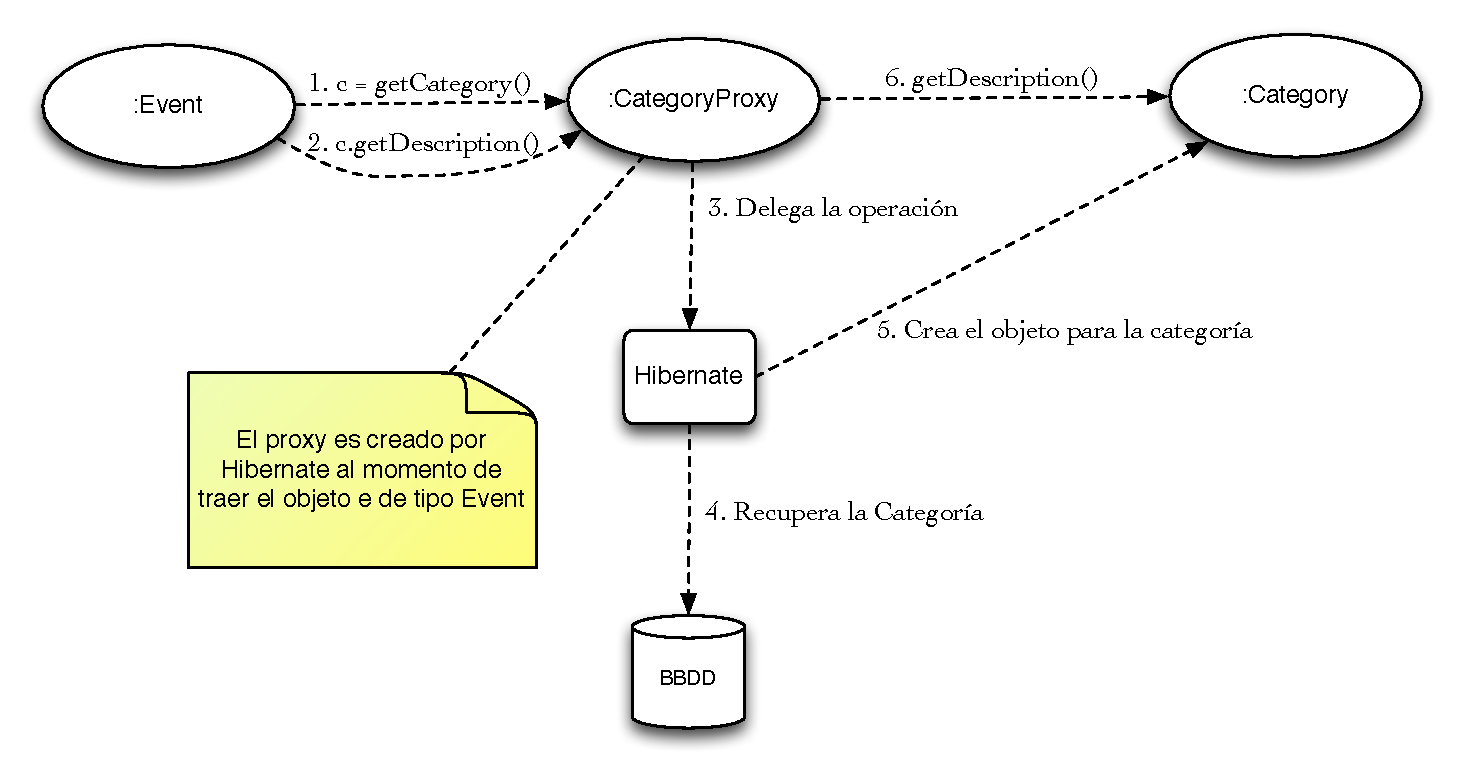
\includegraphics[width=0.8\textwidth]{commit04/img/Proxy.pdf}
  \caption{Uso de proxy en Hibernate}
  \label{fig:c04:Proxy}
\end{figure}	


	Ahora nos toca indicar la relación en la clase \emph{Event}, para poder indicar las categorías, para ello añadimos un atributo del tipo \emph{Category} para añadir la categoría a la que pertenece al igual que los métodos get y set para que hibernate pueda tener acceso a ellos. Para indicar la relación podemos hacer uso de la anotación \emph{ManyToOne} a la que le añadimos dos atributos:
{\setlength{\parskip}{0mm}
\begin{itemize}
	\item \textbf{optional}: Indicamos que es \emph{false} para decir que un evento siempre tiene que pertenecer a una categoría.
	\item \textbf{fetch}: A la hora de que se traiga un objeto evento de la base de datos podemos traer también la categoría a la que pertenece, o no. Si le indicamos que es \emph{FetchType.Lazy}, no traemos el objeto categoría con el que está relacionado, con lo que hibernate mete un objeto proxy del tipo categoría, y en el momento en que se necesite (cuando se quiera acceder a algunos de sus atributos) lo irá buscar a la BBDD (véase la figura \ref{fig:c04:Proxy}). Para que traiga los datos desde un principio hay que especificar \emph{FetchType.EAGER}.
\end{itemize}
}
Una vez que especificamos que el objeto categoría es por la relación MuchosAUno, toca indicar como se mapea. Eso se hace con la anotación \emph{JoinColumn} especificando la columna de la tabla \emph{EVENTS} que se usa como clave foránea (que en este caso se llama \emph{category}).
\begin{lstlisting}[style=java]
//[...]
	private Category category;
//[...]
	@ManyToOne(optional=false, fetch=FetchType.LAZY)
	@JoinColumn(name = "category")
	public Category getCategory() {
		return this.category;
	}
	public void setCategory(Category category) {
		this.category = category;
	}
//[...]
\end{lstlisting}

	También hay que indicar a hibernate la creación de la nueva clase persistente eso se hace añadiendo la información en el archivo \emph{hibernate.cfg.xml} la ubicación de la clase
\begin{lstlisting}[style=xml]
<mapping class="org.example.tutorials.hibernate.hibernateTutorial.domain.Category"/>
\end{lstlisting}

	Ya que tenemos la clase persistente para almacenar las categorías vamos a crear un DAO para poder tener acceso a ellas. La interfaz para el DAO de las categorías queda de la siguiente manera:
\lstinputlisting[style=java]{commit04/code/CategoryDao.java}

	mientras que la implementación del DAO usando hibernate queda:
\lstinputlisting[style=java]{commit04/code/CategoryDaoHibernate.java}

\subsubsection{Probando la relación entre eventos y categorías}\label{sec:c04:EventCategory}
	Para probar la parte codificada tenemos que usar las implementaciones de ambos DAOs, el de categorías y el de eventos. El código se muestra a continuación\footnote{Hay que tener en cuenta que, de la manera en la que se creo las tablas y las restricciones en la BBDD, al eliminar las categorías también se eliminan de la BBDD los eventos y, dependiendo de la aplicación, eso puede no ser lo más adecuado}
\lstinputlisting[style=java]{commit04/code/App.java}

\subsection{Estado del sistema}
	Al final de esta iteración lo que tenemos es algo como lo que se muestra en la figura \ref{fig:c04:UmlClass}.
\begin{figure}[h]
  \centering
    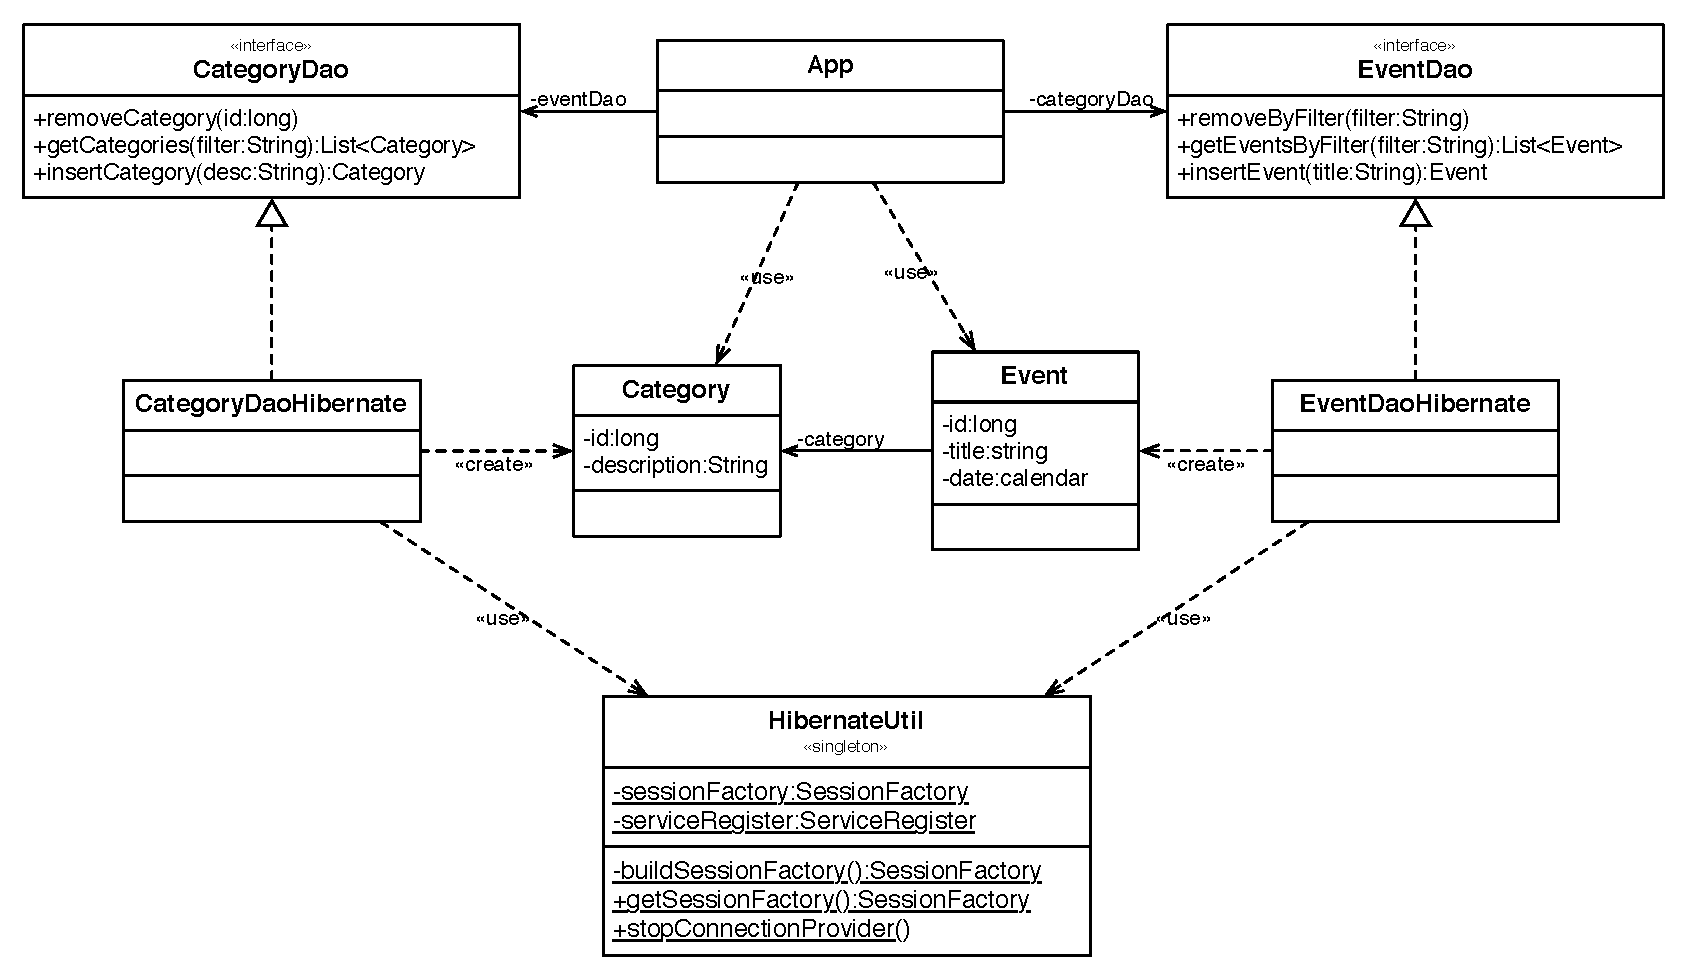
\includegraphics[width=0.95\textwidth]{commit04/img/UmlClass.pdf}
  \caption{Diagrama de clases}
  \label{fig:c04:UmlClass}
\end{figure}	

\section{Commit 5. Un DAO para dominarlos a todos}

	Como podemos ver en el escenario que tenemos en este momento (figura \ref{fig:c04:UmlClass}) hay ciertas operaciones básicas sobre las entidades persistentes que se pueden repetir. Estas operaciones básicas son las operaciones \emph{CRUD}\footnote{\emph{CRUD}: \emph{Create}, \emph{Read}, \emph{Update} y \emph{Delete}}.

\subsection{Diseño del DAO genérico}
	Como hemos podido ver en el apartado \ref{sec:commit2} el patrón DAO proporciona una interfaz para acceso a los datos, donde después dependiendo de la tecnología que se use para la persistencia se tendrá una implementación y otra dependiendo de la tecnología empleada. Esto también se puede realizar con la implementación del DAO genérico, crear una interfaz para dicho DAO y después crear una implementación de dicho DAO, que en este caso será con Hibernate (véase la figura \ref{fig:c05:GenericDao}).

\begin{figure}[h]
  \centering
    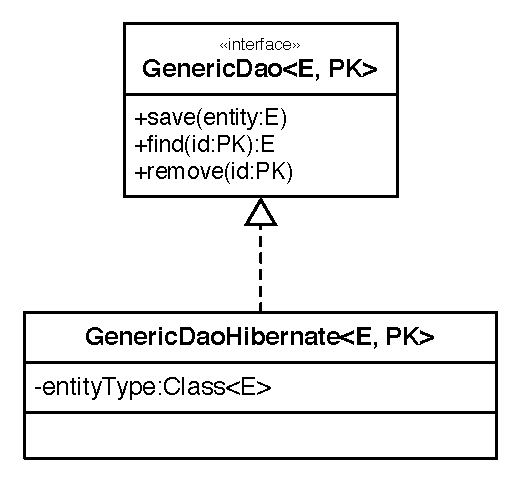
\includegraphics[width=0.3\textwidth]{commit05/img/GenericDao.pdf}
  \caption{Diseño de un DAO genérico}
  \label{fig:c05:GenericDao}
\end{figure}	

\subsection{Implementación del DAO genérico}
La interfaz que se muestra a continuación es definición del DAO genérico:
\lstinputlisting[style=java]{commit05/code/GenericDao.java}

La implementación para el caso de hibernate:
\lstinputlisting[style=java]{commit05/code/GenericDaoHibernate.java}

\subsection{Estado del sistema}
	Como podemos ver tenemos un sistema en donde están definidas las clases persistentes y las definiciones del acceso a los datos, además de una interfaz por defecto que sirve para todas las clases persistentes, mientras que la implementación de Hibernate está por separado y se puede reemplazar facilmente por otro método de persistencia.
	
	Aunque parezca que el diagrama de clases está creciendo de manera incontrolada (figura \ref{fig:c05:UmlClass}), esto no es cierto. El uso de los DAOs nos ayuda a tener una estructura mucho más ordenada lo que ayudará al mantenimiento de la aplicación porque en cada clase sólo está y hace lo que le corresponde. Además lo añadido en esta iteración, el DAO genérico, nos ayuda a ser más rápidos porque ahora cada vez que queramos crear una clase persistente, las operaciones CRUD ya están implementadas y basta con que el DAO extienda de la implementación genérica para poder ser usadas (además de que estamos siguiendo el principio DRY).
	
\begin{figure}[h]
  \centering
    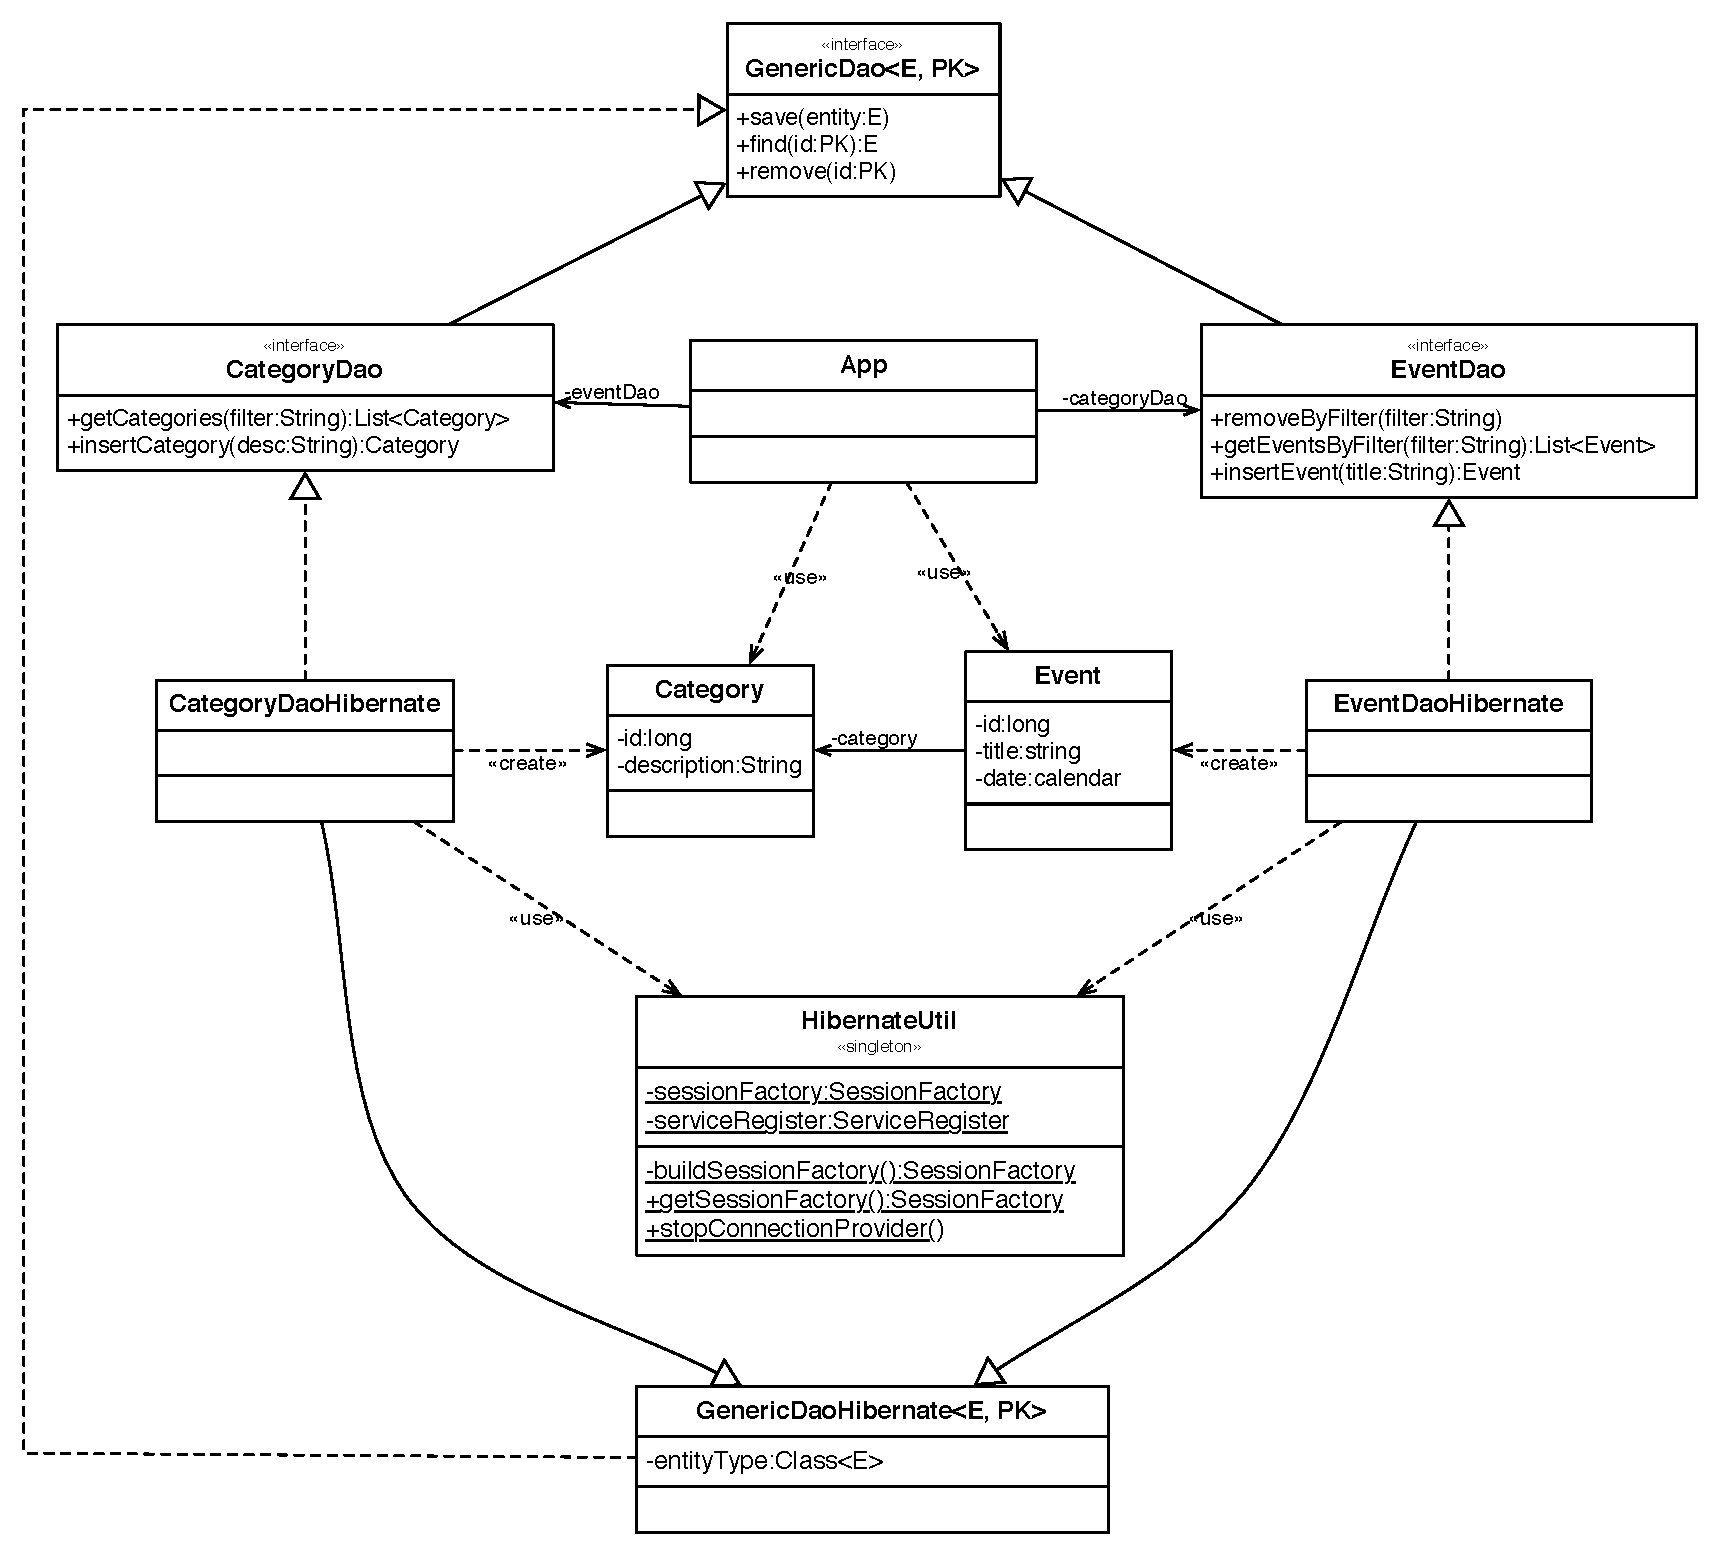
\includegraphics[width=0.95\textwidth]{commit05/img/UmlClass.pdf}
  \caption{Diagrama de clases}
  \label{fig:c05:UmlClass}
\end{figure}	

\section{Commit 6. La BBDD puede tener mucha información}
	En este apartado vamos a evitar una de las malas prácticas que suele tener las personas que hacen pequeñas aplicaciones o aplicaciones que no se testean con las pruebas adecuadas. Una de las cosas que hay que tener en cuenta es la cantidad de información que se puede almacenar en la BBDD.  Si nos fijamos en el código que tenemos en el \emph{Main} del apartado \ref{sec:c04:EventCategory} podemos ver que para la categoría correspondiente a los deportes de agua tenemos 19 eventos, aunque nada impide tener un millón de eventos. Una de las operaciones que se pueden añadir al DAO de la categoría es la de obtener todos los eventos de una categoría. Si el número de elementos que puede tener un conjunto puede ser muy grande, puede hacer que la preparación de las tuplas seleccionadas en la BBDD lleve mucho tiempo, además que le hay que sumar el tiempo de pasar las tuplas de la BBDD a objetos persistentes de Java, además del consumo de memoria que eso puede suponer.
	
	Para solucionar esos problemas se hace uso del patrón \emph{PageByPage} que lo que nos indica es que se traigan los datos poco a poco, por ejemplo de 10 en 10.

\subsection{Implementación del patrón PageByPage}
	Para el ejemplo de devolver los eventos a las categorías basta con añadir a la interfaz \emph{EventDao.java} dos métodos, uno para obtener una lista acotada de eventos y otra para obtener cual es el número total de elementos y poder saber hasta cuando iterar para obtenerlos todos.
\begin{lstlisting}[style=java]
	public long getNumberOfEventsByCategory(long categoryId);
	public List<Event> getEventsByCategory(long categoryId, int start, int size);
\end{lstlisting}

	La implementación de dichos métodos con hibernate, que están en la clase 
\emph{EventDaoHibernate.java}, son de la siguiente manera:
\begin{lstlisting}[style=java]
	@SuppressWarnings("unchecked")
	public List<Event> getEventsByCategory(long categoryId, int start, int size) {
		Session session = HibernateUtil.getSessionFactory().openSession();
    	Transaction transaction = null;
    	
    	List<Event> list = null;
    	try {
    		transaction = session.beginTransaction();
    		
    		Query query = session.createQuery(
    				"SELECT e " +
    				"FROM Event e " +
    				"WHERE e.category.id = :categoryId "+
    				"ORDER BY e.category.description"
    		);
    		
    		list = query
    					.setParameter("categoryId", categoryId)
    					.setFirstResult(start)
    					.setMaxResults(size)
    					.list();
    		
    		transaction.commit();
    	} catch (HibernateException e) {
    		transaction.rollback();
    	} finally {
    		session.close();
    	}
    	
    	return list;
	}
	
	public long getNumberOfEventsByCategory(long categoryId){
		Session session = HibernateUtil.getSessionFactory().openSession();
    	Transaction transaction = null;
    	
    	long size = 0;
    	try {
    		transaction = session.beginTransaction();
    		
    		Query query = session.createQuery(
    				"SELECT COUNT(e) " +
    				"FROM Event e " +
    				"WHERE e.category.id = :categoryId"
    		);
    		
    		size = (long) query.setParameter("categoryId", categoryId).uniqueResult();
    		
    		transaction.commit();
    	} catch (HibernateException e) {
    		transaction.rollback();
    	} finally {
    		session.close();
    	}
    	
    	return size;
	}
\end{lstlisting}

\subsection{Estado del sistema}
	Hay que tener en cuenta que la implementación del patrón PageByPage no es sólo para obtener los elementos de una relación, si no que se ha de implementar en cualquier método que tenga la posibilidad de devolver un conjunto grande de datos.
	
\begin{figure}[h]
  \centering
    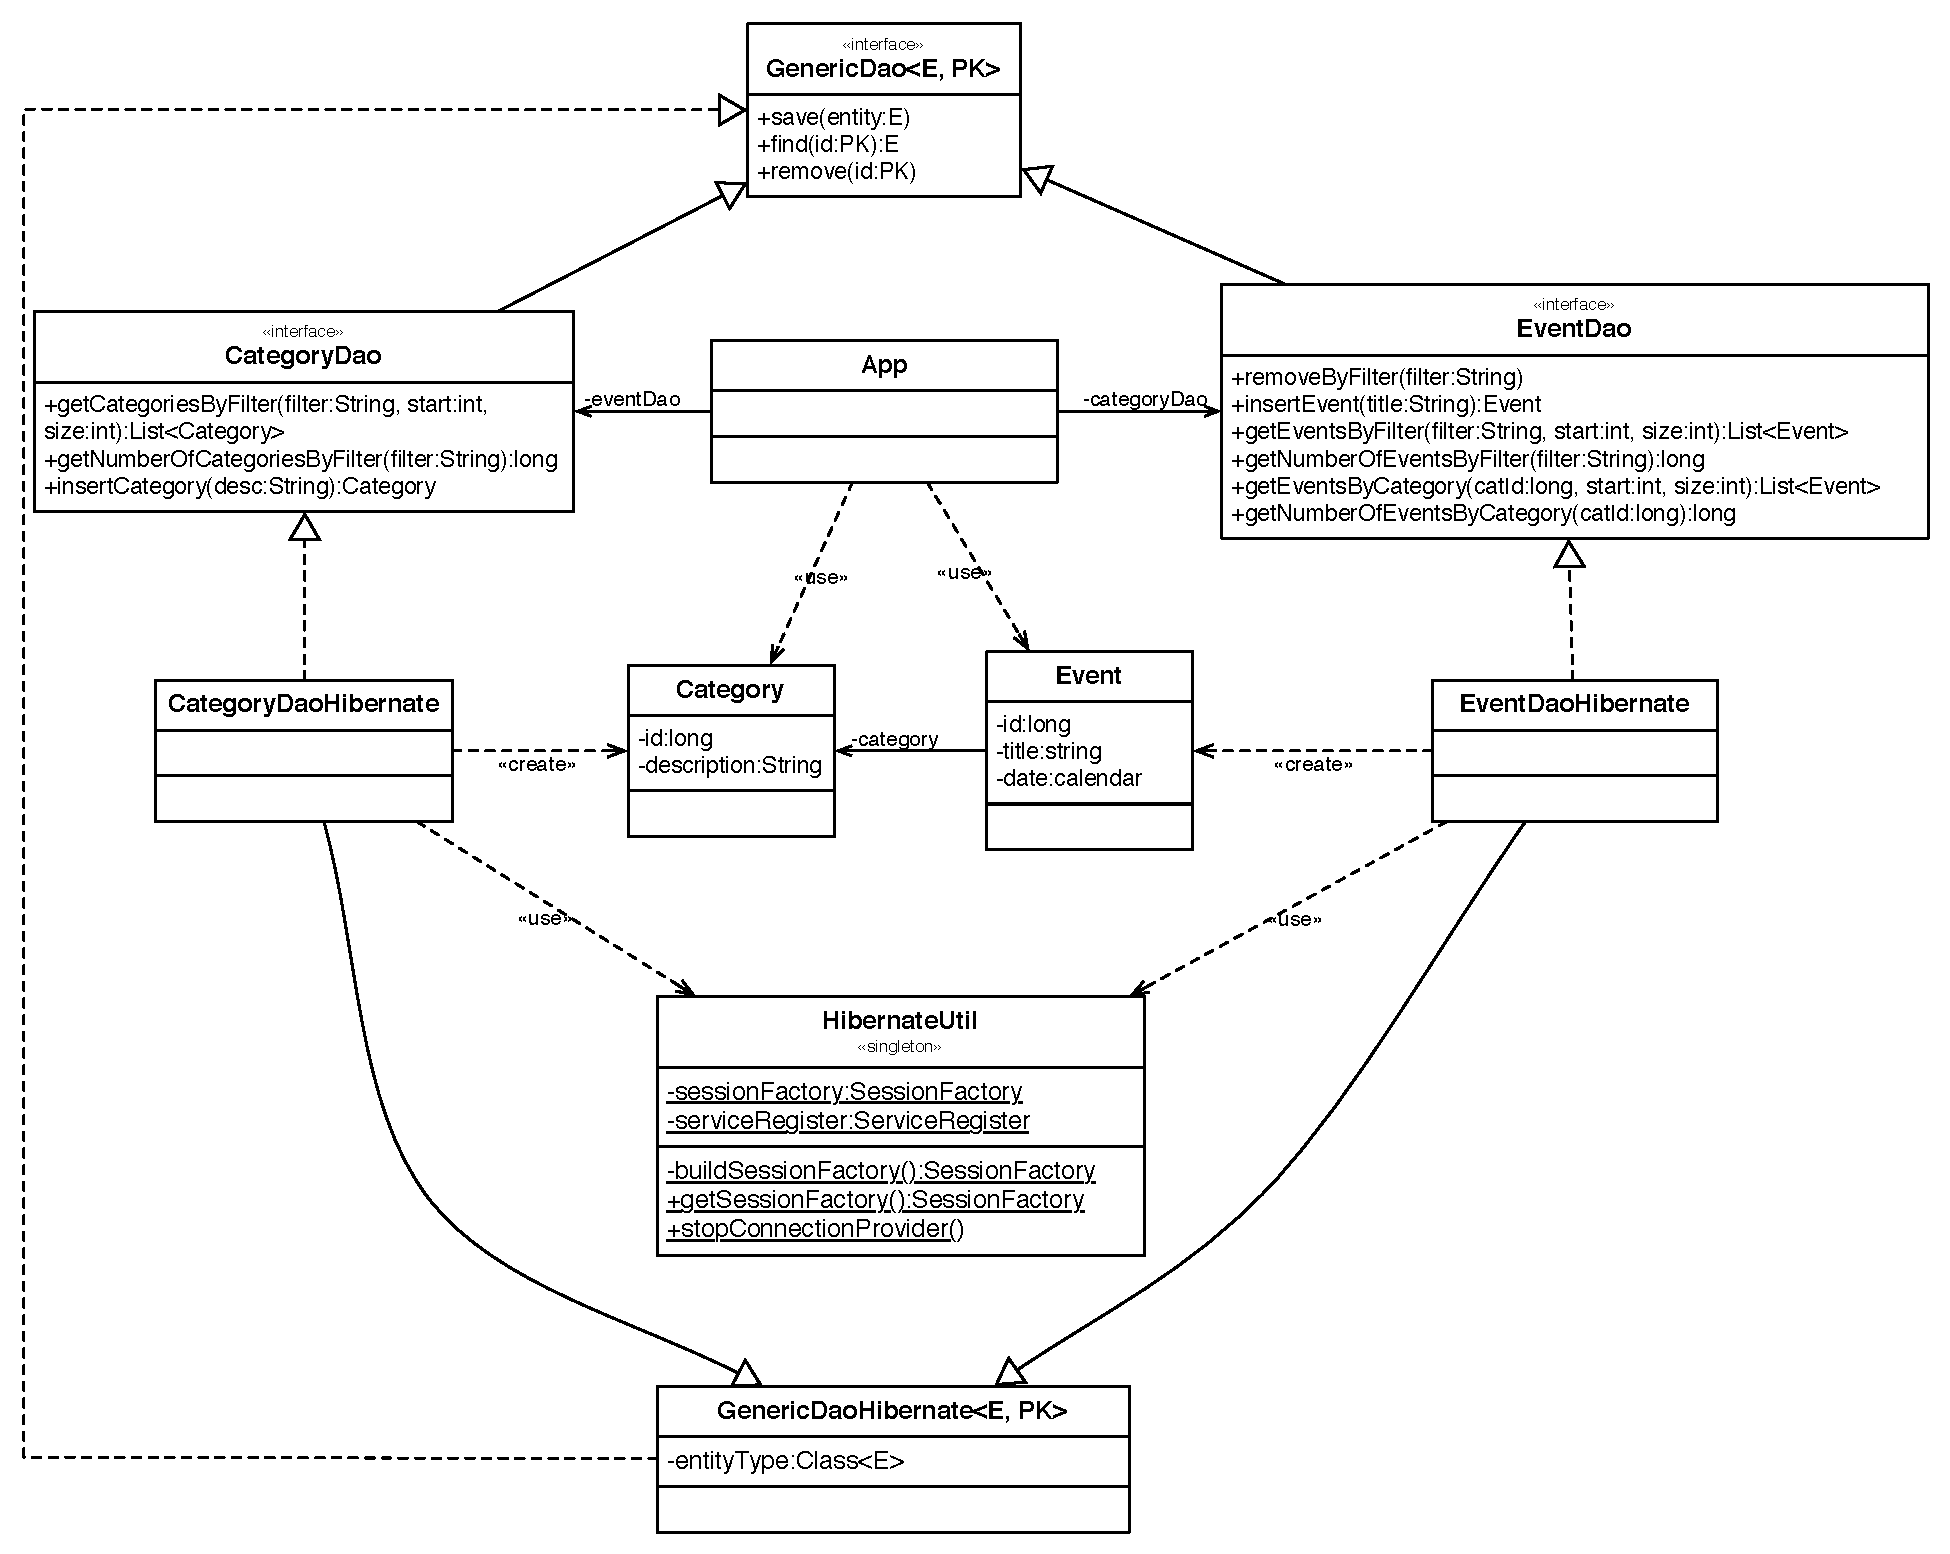
\includegraphics[width=0.95\textwidth]{commit06/img/UmlClass.pdf}
  \caption{Diagrama de clases}
  \label{fig:c05:UmlClass}
\end{figure}	

\clearpage
\newpage
{\setlength{\parskip}{0mm}\listoffigures}

% Bibliografía.
%-----------------------------------------------------------------
\clearpage

\renewcommand{\bibname}{Referencias}
\begin{thebibliography}{99}
\bibitem{HibernateData}
Tipos de datos de Hibernate

\url{http://docs.jboss.org/hibernate/orm/4.3/manual/en-US/html/ch06.html\#types-value}

\url{http://www.tutorialspoint.com/hibernate/hibernate\_mapping\_types.htm}
\bibitem{Dao}
Patrón Dao (\textit{Data Access Object})

\url{http://gl.wikipedia.org/wiki/Data_access_object}
\end{thebibliography}

\end{document}